\subsection{Integrations}

\begin{itemize}
\item MARBL
\item ARES
\item AMRex: Warpx, Pele, NYX
\item SW4
\end{itemize}



\subsection{MARBL:Big Laser Tiny Box}
\fix{Placeholder text.}
Figures~\ref{img:radkh} and \ref{img:radkh_xray} show images create from
a simulation of a real work experiment, where scientists destroyed a tiny box
with a powerful laser.
%
This is a important use case due to the impending tiny box invasion.

\begin{figure}
\centering
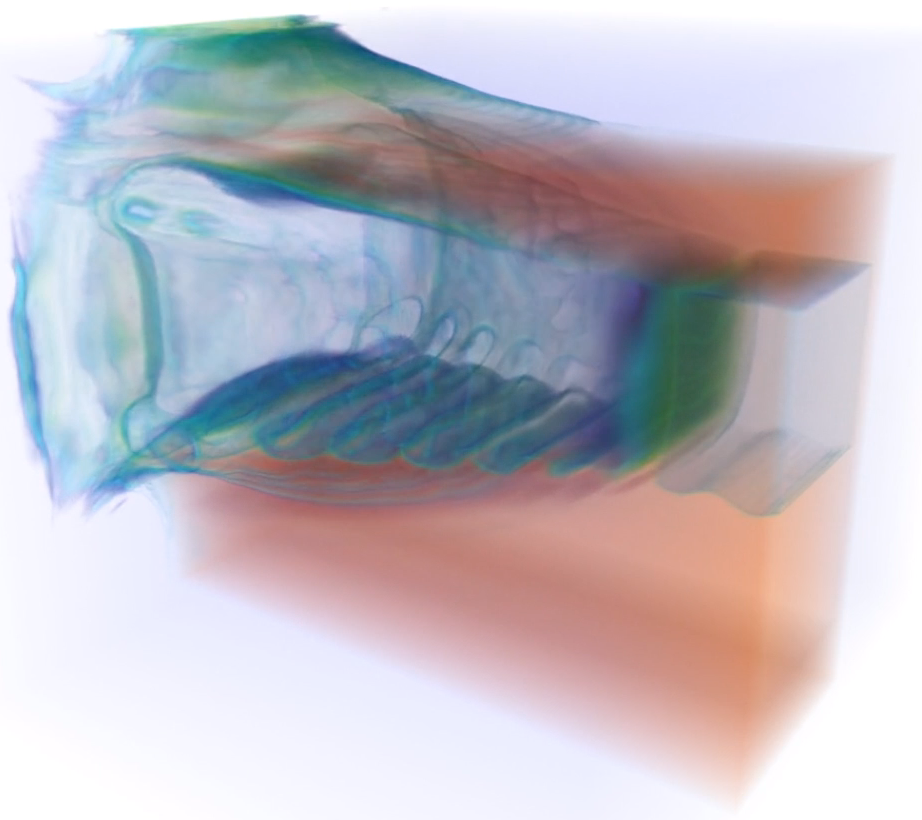
\includegraphics[width=0.6\textwidth]{images/radkh}
\caption{\label{img:radkh} Image of a comically sized lazer destroying a small box.}
\end{figure}

\begin{figure}
\centering
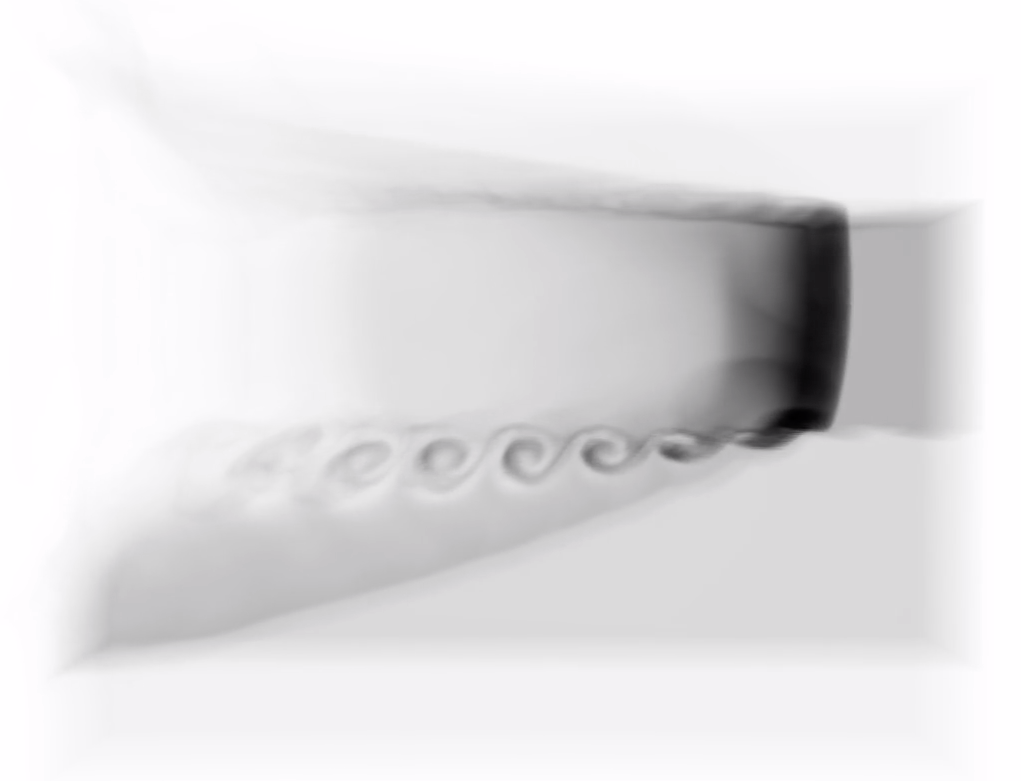
\includegraphics[width=0.6\textwidth]{images/radkh_xray}
\caption{\label{img:radkh_xray}Simulated radiograph of a comically sized lazer destroying a small box.}
\end{figure}

\subsection{Ares: Milk-Chocolate Mixing (Colorized)}

The image in Figure~\ref{img:icf} was created in situ using
Ascent, which performed its tasks using
the same resources as the simulation code, in this
case 4096 nodes and 16,384 GPUs.

\begin{figure}
\centering
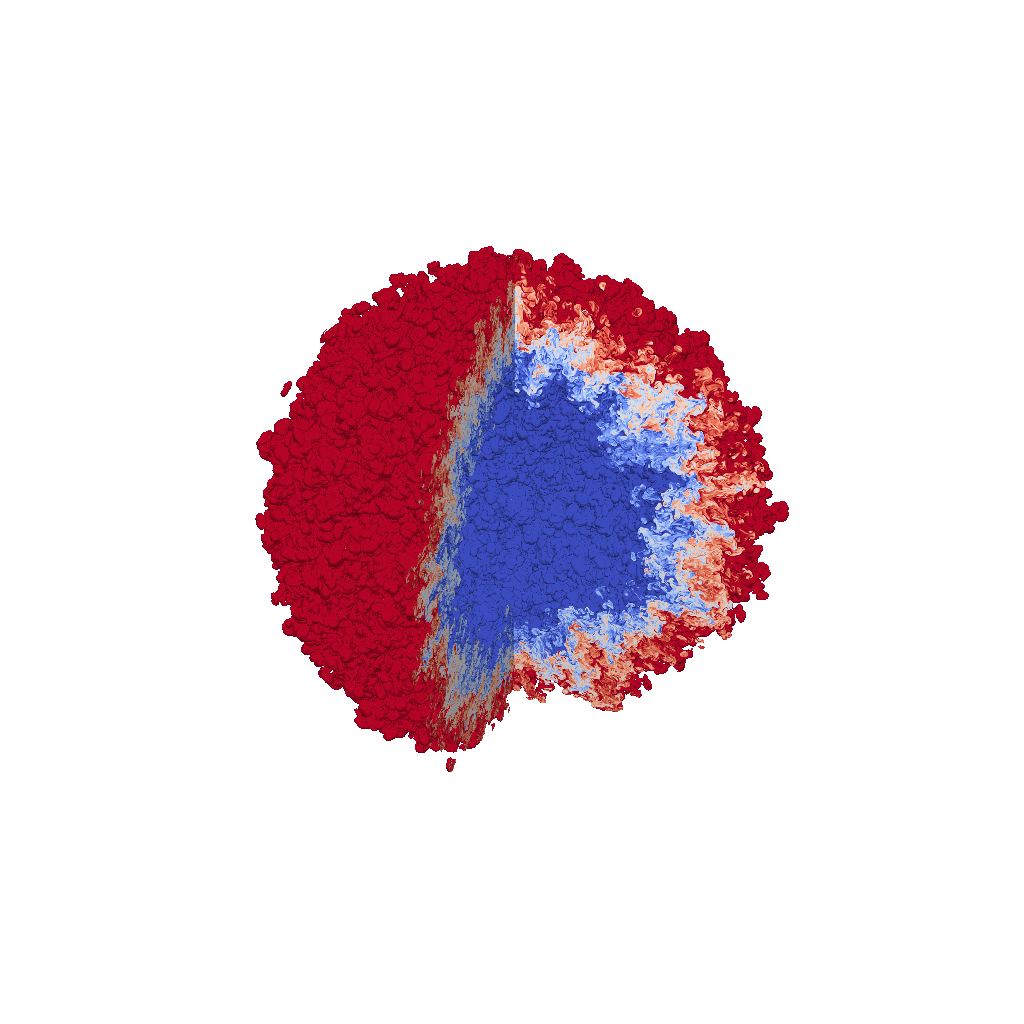
\includegraphics[trim={ 0 8cm 0 7cm},width=0.9\textwidth]{images/mixing_ball}
\caption{\label{img:icf}
This image is of an idealized Inertial Confinement
Fusion (ICF) simulation of a Rayleigh–Taylor instability
with two fluids mixing in a spherical geometry.
}
\end{figure}
